Our everyday experience might lead us to believe that the eyes are sensory organs developed completely separate from the brain but, in fact, the retina is an extension of the brain that performs spatio-temporal compression of a continuous flow of ``images'' of the world~\cite{eye-brain-vision-hubel1995}.

The eye is composed of many parts that resemble a mechanical camera (Figure~\ref{fig:vision:eye}). The cornea is a transparent film that protects the frontal part of the eye, it may be seen as part of a membrane that encloses the eye. The lens is in charge of focusing light rays into the retina, the latter acts as a complex sensor which will be described further in the following paragraphs. The pupil and the iris act as a camera's aperture mechanism, the amount of light is regulated by broadening or reducing the diameter of the pupil. After the light rays have been encoded into a neural representation, the optic nerve transfers the information to the Lateral Geniculate Nucleus (LGN) and from there to the visual portion of the cortex. A huge difference between a camera and the eye is that the latter maintains a continuous stream of information unlike the frame-based nature of cameras.

\begin{figure}[htb]
  \begin{center}
    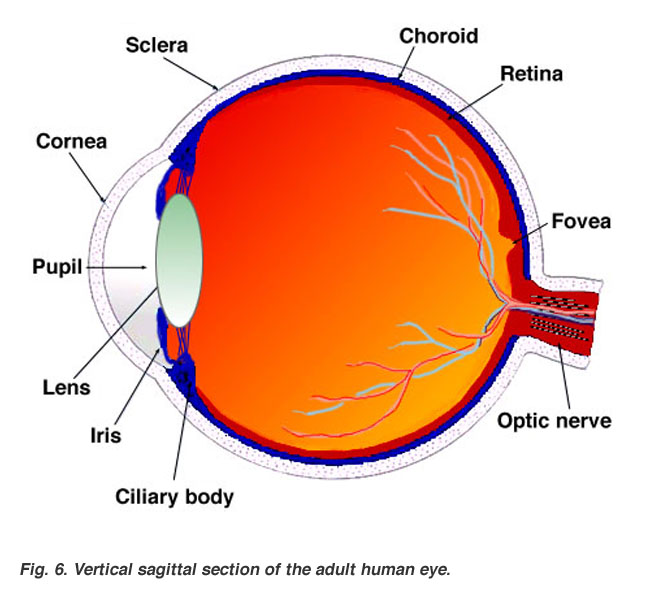
\includegraphics[width=0.5\textwidth]{simple-eye-anatomy}
    \caption{Simplified anatomy of the eye~\cite{webvision-images}.}
    \label{fig:vision:eye}
  \end{center}
\end{figure}

The retina is organized in layers of cell bodies and nerves,  Figure~\ref{fig:vision:simple-retina} shows a simplified version of the retina's anatomy~\cite{webvision-simple-retina}. Light enters the eye and has to travel all the way to the deepest part of the retina (right of Fig.~\ref{fig:vision:simple-retina}) to be sensed by the photoreceptors. 

\begin{figure}[h]
  \begin{center}
    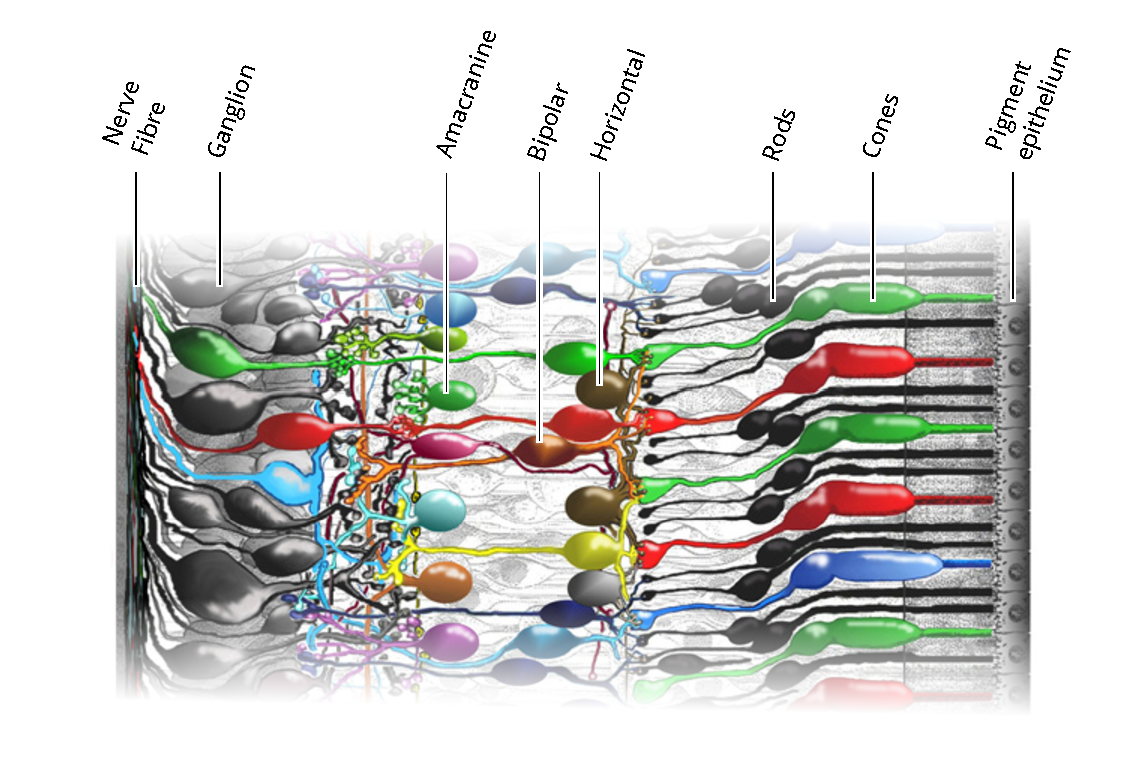
\includegraphics[width=0.7\textwidth]{retina-simple}
    \caption{Simple anatomy of the retina, adapted from~\cite{webvision-images}.}
    \label{fig:vision:simple-retina}
  \end{center}
\end{figure}

Photoreceptors transform light into an electrical signal. Colour is perceived by special type of receptors \emph{cones} and for low-light conditions and higher contrast sensitivity the retina uses \emph{rods}. Many mammals have retinas with more rods than cones. For primates the retina has two almost dual sensor zones. Most of the photosensitive area has more rods than cones; a tiny region called the \emph{foveal pit} has almost no rods, it's densely packed with cones for high-resolution vision and is virtually blind when there is not enough light~\cite{eye-brain-vision-hubel1995}.

The precise function of horizontal, bipolar and amacranine is still a matter of debate and research. What is known is that \textbf{horizontal} cells average spatially the input from photoreceptors and transmit to bipolar, which in turn output to ganglion cells. Horizontal cells also send a feedback signal to the photoreceptors, the reason of the latter might be to adapt to different light conditions. \textbf{Bipolar} cells are called like that because the have outputs both to ganglion cells and photoreceptors. These first cell types use analog signals and feed ganglion cells which have a \emph{centre-surround} behaviour~\cite{eye-brain-vision-hubel1995,thompson2000brain}. Figure~\ref{fig:vision:centre-surround} illustrates the reaction of the two variants of centre-surround cells to different inputs.

\begin{figure}[h]
  \begin{center}
    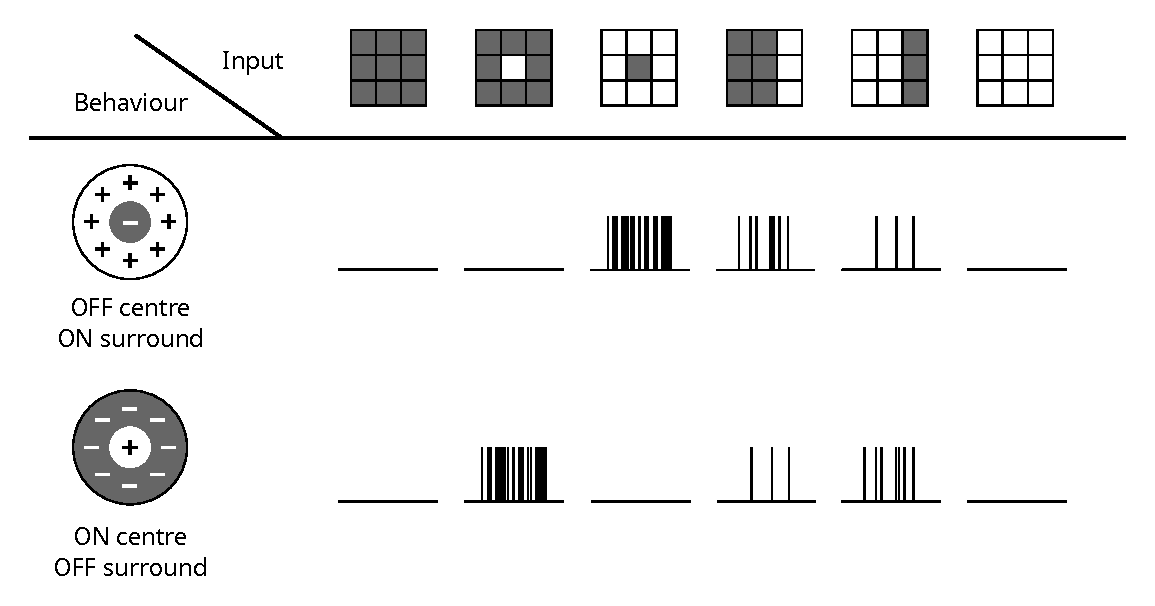
\includegraphics[width=0.7\textwidth]{centre-surround}
    \caption{Responses of centre-surround cells to different types of input.}
    \label{fig:vision:centre-surround}
  \end{center}
\end{figure}


\textbf{Ganglion} cells take input from bipolar cells, some will form the surround (signal adapted by horizontal cells) and others the centre (pure signal from the photoreceptors). The centre-surround behaviour has been modelled by many authors using Laplacian of Gaussians or \emph{Difference of Gaussians}. The output of ganglion cells are action potentials which are transmitted by the nerve fibre, which are the ganglion's axons, into the lateral geniculate nucleus.

It's likely that most of the information sensed by the retina is redundant, this would keep the eyes working adequately even if some cells cease to function. To avoid saturation of nerve fibres and over-representation lateral inhibition might play a big role~\cite{basab-model,thorpe-rate-coding-theory,field-sensory-coding}. The use of centre-surround responses in the retina is believed to help the eye overcome difference in lightning conditions, because the response comes from the contras comparison between photoreceptors.


